\documentclass[11pt]{charter}

\usepackage{graphicx}
\usepackage{calc}
\usepackage[T1]{fontenc}

% El títulos de la memoria, se usa en la carátula y se puede usar el cualquier lugar del documento con el comando \ttitle
\titulo{Realidad Aumentada para la optimización de procedimientos \textit{batch} en la industria} 
	
% Nombre del posgrado, se usa en la carátula y se puede usar el cualquier lugar del documento con el comando \degreename
\posgrado{Carrera de Especialización en Sistemas Embebidos} 
%\posgrado{Carrera de Especialización en Internet de las Cosas} 
%\posgrado{Carrera de Especialización en Intelegencia Artificial}
%\posgrado{Maestría en Sistemas Embebidos} 
%\posgrado{Maestría en Internet de las cosas}

% Tu nombre, se puede usar el cualquier lugar del documento con el comando \authorname
\autor{Iván Szkrabko} 

% El nombre del director y co-director, se puede usar el cualquier lugar del documento con el comando \supname y \cosupname y \pertesupname y \pertecosupname
\director{Leandro Lanzieri}
\pertenenciaDirector{UTN} 
% FIXME:NO IMPLEMENTADO EL CODIRECTOR ni su pertenencia
\codirector{} % si queda vacio no se deberíá incluir 
\pertenenciaCoDirector{}

% Nombre del cliente, quien va a aprobar los resultados del proyecto, se puede usar con el comando \clientename y \empclientename
\cliente{Alejandro Carrasco}
\empresaCliente{ABB}

% Nombre y pertenencia de los jurados, se pueden usar el cualquier lugar del documento con el comando \jurunoname, \jurdosname y \jurtresname y \perteunoname, \pertedosname y \pertetresname.
\juradoUno{Nombre y Apellido (1)}
\pertenenciaJurUno{pertenencia (1)} 
\juradoDos{Nombre y Apellido (2)}
\pertenenciaJurDos{pertenencia (2)}
\juradoTres{Nombre y Apellido (3)}
\pertenenciaJurTres{pertenencia (3)}
 
\fechaINICIO{27 de junio de 2020}		%Fecha de inicio de la cursada de GdP \fechaInicioName
\fechaFINALPlanificacion{22 de Agosto de 2020} 	%Fecha de final de cursada de GdP
\fechaFINALTrabajo{22 de diciembre de 2020}		%Fecha de defensa pública del trabajo final


\begin{document}

\maketitle
\thispagestyle{empty}
\pagebreak


\thispagestyle{empty}
{\setlength{\parskip}{0pt}
\tableofcontents{}
}
\pagebreak


\section{Registros de cambios}
\label{sec:registro}


\begin{table}[ht]
\label{tab:registro}
\centering

\begin{tabularx}{\linewidth}{@{}|c|X|c|@{}}
\hline
\rowcolor[HTML]{CBCEFB} 
Revisión & \multicolumn{1}{c|}{\cellcolor[HTML]{CBCEFB}Detalles de los cambios realizados} & Fecha\\ \hline
1.0      & Creación del documento                                                          
		 & 27/06/2020 \\ \hline
1.1      & Primera versión, completo hasta punto 6                                                                                         	 	 & 10/07/2020 \\ \hline
1.2      & Completo hasta punto 11 																						   	 & 30/07/2020 \\ \hline
1.3      & Completo todo el documento 																						 & 08/08/2020 \\ \hline  
1.4      & Agrego historias de usuarios 																				     & 10/08/2020 \\ \hline                                                                   
\end{tabularx}
\end{table}

\pagebreak



\section{Acta de constitución del proyecto}
\label{sec:acta}

\begin{flushright}
Buenos Aires, \fechaInicioName
\end{flushright}

\vspace{2cm}

Por medio de la presente se acuerda con el Ing.\authorname\hspace{1px} que su Trabajo Final de la \degreename\hspace{1px} se titulará ``\ttitle'', consistirá esencialmente en el prototipo preliminar de una aplicación de software para la supervisión y control de procesos \textit{batch} en la industria, y tendrá un presupuesto preliminar estimado de 640 hs de trabajo y \$ 5000, con fecha de inicio \fechaInicioName\hspace{1px} y fecha de presentación pública \fechaFinalName.

Se adjunta a esta acta la planificación inicial.

\vfill

% Esta parte se construye sola con la información que hayan cargado en el preámbulo del documento y no debe modificarla
\begin{table}[ht]
\centering
\begin{tabular}{ccc}
\begin{tabular}[c]{@{}c@{}}Ariel Lutenberg \\ Director posgrado FIUBA\end{tabular} &  & \begin{tabular}[c]{@{}c@{}}\clientename \\ \empclientename \end{tabular} \vspace{2.5cm} \\ 
\multicolumn{3}{c}{\begin{tabular}[c]{@{}c@{}} \supname \\ Director del Trabajo Final\end{tabular}} \vspace{2.5cm} \\
\begin{tabular}[c]{@{}c@{}}\jurunoname \\ Jurado del Trabajo Final\end{tabular}     &  & \begin{tabular}[c]{@{}c@{}}\jurdosname\\ Jurado del Trabajo Final\end{tabular}  \vspace{2.5cm}  \\
\multicolumn{3}{c}{\begin{tabular}[c]{@{}c@{}} \jurtresname\\ Jurado del Trabajo Final\end{tabular}} \vspace{.5cm}                                                                     
\end{tabular}
\end{table}




\section{Descripción técnica-conceptual del proyecto a realizar}
\label{sec:descripcion}

\begin{consigna}{black}
El presente proyecto consiste en desarrollar una interfaz de realidad aumentada, para que los operadores de plantas industriales puedan interactuar con un sistema de control distribuido de una manera práctica e innovadora. La solución hace foco en la capacitación de los operadores, mediante el uso de rutinas \textit{batch}. Las cuales permiten realizar una tarea compleja, sub dividiéndola en tareas simples organizadas de manera secuencial. Con esto se logra evitar que los procedimientos de trabajo se alteren y sufran desvíos. El objetivo es guiar al operador a través de los distintos procedimientos industriales, como pueden ser, arranques o paradas de emergencia en equipos críticos como hornos, calderas y reactores. La solución se implementará sobre un equipo de realidad aumentada de última tecnología de Microsoft denominado HoloLens2. Su plataforma de desarrollo se divide en dos áreas. Por un lado se encuentran las interfaces visuales, las cuales se diseñan en Unity3D, que es una conocida plataforma para el desarrollo de videojuegos. Por otro lado se tiene el backend, este se desarrollará en .NET utilizando CSharp como lenguaje de programación. La aplicación embebida se comunicará con un servidor local a través de una APIrest, y desde el mismo se enviarán los datos pertinentes al sistema de control distribuido de ABB, a través del \textit{standard} industrial OPC (\textit{Open Platform Communications}).  

En la Figura \ref{fig:esquema_inicial} se puede observar de izquierda a derecha el flujo de la información, que comienza con un \textit{input} en la interfaz visual por parte del operador y termina con una acción determinada en el sistema de control.

\vspace{25px}

\begin{figure}[htpb]
    \centering
    \def\svgwidth{\columnwidth}
    \fontsize{8}{5}\fontencoding{T1}\fontfamily{lmss}\fontseries{eb}\selectfont
%	\def\svgscale{1}
    \input{Esquema_inicial.pdf_tex}
	\caption{Diagrama en bloques simplificado}
	\label{fig:esquema_inicial}
\end{figure}

\vspace{25px}

\end{consigna}


\section{Identificación y análisis de los interesados}
\label{sec:interesados}

\begin{consigna}{black} 
\begin{table}[ht]
%\caption{Identificación de los interesados}
%\label{tab:interesados}
\begin{tabularx}{\linewidth}{@{}|l|X|X|l|@{}}
\hline
\rowcolor[HTML]{CBCEFB} 
Rol           & Nombre y Apellido & Organización 	& Puesto 					\\ \hline
Auspiciante   & Víctor Toledo     & ABB         	& Gerente de Operaciones	\\ \hline
Cliente       & \clientename      &\empclientename	& Gerente de Ingeniería     \\ \hline
Impulsor      & Guillermo Lamana  & ABB           	& Project Manager       	\\ \hline
Responsable   & \authorname       & FIUBA        	& Alumno 					\\ \hline
Orientador    & \supname	      & \pertesupname 	& Director Trabajo final    \\ \hline
\end{tabularx}
\end{table}
 
Análisis de los interesados:
\begin{itemize}
\item Auspiciante: es riguroso y exigente con la utilización de los recursos y el tiempo.
\item Cliente: es detallista y busca que el producto sea perfecto.
\item Impulsor: es una persona que tiene además un rol de facilitador.
\item Orientador: será una fuente valiosa de consulta.
\end{itemize}

\end{consigna}



\section{1. Propósito del proyecto}
\label{sec:proposito}

\begin{consigna}{black}
El propósito de este proyecto es innovar en la interacción entre los operadores y los sistema de control distribuidos, para impulsar nuevas soluciones en el área de la automatización industrial. Se busca explorar las oportunidades que ofrece la realidad aumentada para mejorar y optimizar las tareas de los operadores, además de agilizar el entrenamiento de nuevos operarios y mejorar la seguridad para procedimientos bajo situaciones de emergencia.
\end{consigna}

\section{2. Alcance del proyecto}
\label{sec:alcance}

\begin{consigna}{black}
\textbf{El alcance del proyecto contempla:}
\begin{itemize}
\item Desarrollar una interfaz visual para el HoloLens2 que permita realizar el seguimiento de procesos \textit{batch} y rutinas de emergencia.
\item Desarrollar una interfaz de comunicación entre el HoloLens2 y un servidor web a través de una APIrest.
\item Desarrollar una interfaz de comunicación OPC entre el servidor web y el sistema de control.
\item Implementar lecturas de códigos QR para lograr el reconocimiento de equipos en planta.
\item Implementar un modo de visualización donde los elementos físicos de planta se complementen con la información del sistema de control, para indicar al operador el estado de cada elemento y sus propiedades en el sistema.
\item Implementar visualización de despieces mecánicos para guiar a los operadores en las tareas de mantenimiento.
\end{itemize}

\textbf{El alcance del proyecto no incluye:}
\begin{itemize}
\item Aquellas funcionalidades que no se encuentren contempladas dentro del alcance definido.
\end{itemize}
\end{consigna}


\section{3. Supuestos del proyecto}
\label{sec:supuestos}

\begin{consigna}{black}
Para el desarrollo del presente proyecto se supone que:

\begin{itemize}
\item Se dispone de 48 hs semanales para dedicar al desarrollo de la solución
\item Se tiene acceso al HoloLens2 durante el desarrollo de la solución
\end{itemize}

\end{consigna}

\section{4. Requerimientos}
\label{sec:requerimientos}

\begin{consigna}{black}
A continuación se listan los requerimientos en base a las distintas etapas de la solución:

\begin{enumerate}
\item Requerimientos asociados al desarrollo de la interfaz visual:
	\begin{enumerate}
	\item La interfaz debe ser intuitiva y simple.
	\item El idioma definido es Español.
	\end{enumerate}
\item Requerimientos asociados al desarrollo de lógica en .NET:
	\begin{enumerate}
	\item La aplicación debe ser fluida y responder sin demoras apreciables por el operador, estableciéndose así el límite máximo de espera en 2 segundos.
	\item La aplicación debe poder hacer operaciones GET y POST sobre un servidor web, ya sea local o en la nube.
	\end{enumerate}
\item Requerimientos asociados a la API rest:
	\begin{enumerate}
	\item La API no será de acceso público, solo podrá ser consultada por las aplicaciones que poseen un \textit{token} de seguridad.
	\end{enumerate}
\item Requerimientos asociados a la interfaz de comunicación con el sistema de control:	
	\begin{enumerate}	
	\item La solución debe poder consultar una serie de datos específicos a elección, de los elementos que pertenecen al sistema de control.
	\item La comunicación debe cumplir con el \textit{standard} OPC.
	\end{enumerate}
\end{enumerate}

\end{consigna}

\section{Historias de usuarios (\textit{Product backlog})}
\label{sec:backlog}
\begin{consigna}{black}
La Ponderación tendrá un rango de calificación de 1 a 5 y se basará en el esfuerzo de desarrollo, donde 1 implica el máximo esfuerzo.

La Prioridad tendrá un rango de calificación de 1 a 5 y se basará en la funcionalidad que aporta al sistema, donde 1 implica máxima prioridad.
\end{consigna}

\begin{itemize}
\item Historia 1
\begin{itemize}
\item Ponderación: 1
\item Prioridad: 1
\end{itemize}
Como Usuario, quiero poder visualizar datos del sistema de control como bombas, motores, válvulas y tanques.

\item Historia 2
\begin{itemize}
\item Ponderación: 3
\item Prioridad: 1
\end{itemize}
Como Usuario, quiero poder usar el sistema en un ámbito industrial.

\item Historia 3
\begin{itemize}
\item Ponderación: 2
\item Prioridad: 2
\end{itemize}
Como Usuario, quiero poder usar la solución con sistemas de control de varios proveedores.

\item Historia 4 
\begin{itemize}
\item Ponderación: 3
\item Prioridad: 2
\end{itemize}
Como Usuario, quiero tener un interfaz de manejo sencilla y práctica.

\item Historia 5 
\begin{itemize}
\item Ponderación: 2
\item Prioridad: 2
\end{itemize}
Como Usuario, quiero que la infraestructura necesaria para implementar la solución sea \textit{on-premise}.

\end{itemize}


\section{5. Entregables principales del proyecto}
\label{sec:entregables}

\begin{consigna}{black}
Se entregarán los siguientes elementos:
\begin{itemize}
\item Manual de uso
\item Diagrama esquemático
\item Informe final
\end{itemize}

\end{consigna}

\section{6. Desglose del trabajo en tareas}
\label{sec:wbs}

\begin{consigna}{black}
Se divide el trabajo del proyecto en tareas y subtareas. Para facilitar el seguimiento, ninguna subtarea
consumirá más de 40 horas:

\begin{enumerate}
\item Investigación (Total: 24 hs)
	\begin{enumerate}
	\item Búsqueda de referencias a proyectos similares. (8 hs)
	\item Búsqueda y análisis de \textit{frameworks} útiles para desarrollar las soluciones.  (8 hs)
	\item Investigación de los servicios de Azure, para integrar al desarrollo. (8 hs)
	\end{enumerate}
\item Desarrollo de la interfaz visual: (Total: 88 hs)
	\begin{enumerate}
	\item Diseño de interfaz para la lectura de códigos QR. (16 hs)
	\item Diseño de interfaz para visualización de la información de los elementos del sistema de control. (16 hs)
	\item Diseño de interfaz para guiar al operador a través de los distintos pasos del procedimiento \textit{batch}. (40 hs)
	\item Pruebas, correcciones y mejoras. (16 hs)
	\end{enumerate}
\item Desarrollo de la lógica para la interfaz visual: (Total: 136 hs)
	\begin{enumerate}
	\item Desarrollo de la lógica para realizar las lecturas de códigos QR. (40 hs)
	\item Desarrollo de la lógica para realizar la interacción del operador con los datos del sistema. (32 hs)
	\item Desarrollo de la lógica para guiar al operador a través de los distintos pasos del procedimiento \textit{batch}. (32 hs)
	\item Pruebas, correcciones y mejoras. (32 hs)
	\end{enumerate}
\item Desarrollo de la API Rest (Total: 152 hs)
	\begin{enumerate}
	\item Investigación de distintas tecnologías. (16 hs)
	\item Desarrollo de la solución:
		\begin{enumerate}
			\item Programación de \textit{endpoints}. (40 hs)
			\item Implementación de medidas de seguridad de la API. (40 hs)
			\item \textit{Hosting} de la API. (40 hs)
		\end{enumerate}
	\item Pruebas, correcciones y mejoras. (16 hs)
	\end{enumerate}
\item Desarrollo de la interfaz de comunicación OPC (Total: 160 hs)
	\begin{enumerate}
	\item Investigación de \textit{frameworks} y análisis del protocolo (40 hs)
	\item \textit{Deploy} del cliente OPC (40 hs)
	\item Desarrollo de la comunicación con el server OPC (40 hs)
	\item Pruebas, correcciones y mejoras. (40 hs)
	\end{enumerate}

\item Pruebas integrales (Total: 32 hs)

\item Documentación (Total: 32 hs)

\item Presentaciones al cliente (Total: 16 hs)
\end{enumerate}

Cantidad total de horas: (640 hs) 

\end{consigna}

\section{7. Diagrama de Activity On Node}
\label{sec:AoN}

\begin{consigna}{black}
Los tiempos de las tareas en la Figura \ref{fig:aon} se encuentran expresados en horas:

\begin{figure}[H]
    \centering
    \def\svgwidth{\columnwidth}  
    \fontsize{7}{5}\fontencoding{T1}\fontfamily{lmss}\fontseries{eb}\selectfont
%	\def\svgscale{1}
    \input{aon.pdf_tex}
	\caption{Diagrama Activity On Node}
	\label{fig:aon}
\end{figure}

En el AON se marco con color rojo el considerado camino crítico del proyecto. Si bien hay un conjunto de tareas en paralelo a lo largo del camino crítico, las tareas que atraviesa son las que se consideran de mayor riesgo y dificultad. 

\end{consigna}

\section{8. Diagrama de Gantt}
\label{sec:gantt}

\begin{consigna}{black}
Se elaboró el siguiente diagrama considerando una cantidad de 15 horas semanales efectivas de trabajo:

\begin{figure}[H]
 \centering
 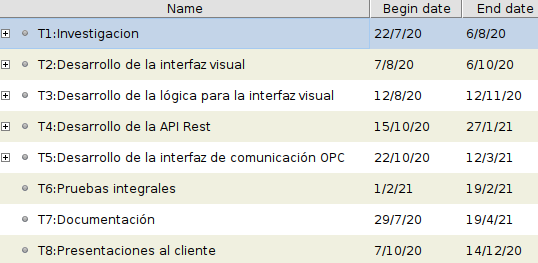
\includegraphics[width=10cm]{gantt_1.png}
 \caption{Fechas asociadas a las tareas}
\end{figure}



\begin{figure}[H]
 \centering
 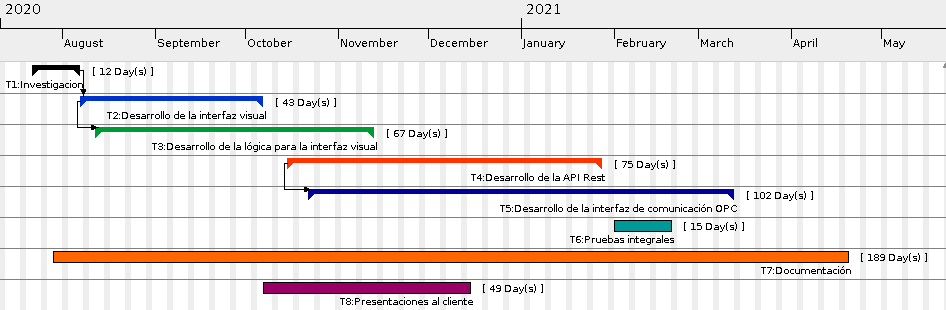
\includegraphics[width=17cm]{gantt_2.png}
 \caption{Diagrama de Gantt}
 \label{figure:Diagrama de Gantt}
\end{figure}

\end{consigna}

\section{9. Matriz de uso de recursos de materiales}
\label{sec:recursos}

\begin{table}[H]
\centering
\setlength\arrayrulewidth{1pt}
\begin{tabular}{|c|c|c|c|}
\hline
\rowcolor[HTML]{CBCEFB} 
\cellcolor[HTML]{CBCEFB}                             & \cellcolor[HTML]{CBCEFB}    & \multicolumn{2}{c|}{\cellcolor[HTML]{CBCEFB} \textbf {Recursos Requeridos}} \\ \cline{3-4} 
\rowcolor[HTML]{CBCEFB} 
\multirow{-2}{*}{\cellcolor[HTML]{CBCEFB} \textbf {Código WBS}} & \multirow{-2}{*}{\cellcolor[HTML]{CBCEFB} \textbf {Nombre Tarea}} & \textbf {PC}                          & \textbf {HoloLens2}                          \\ \hline
\cellcolor[HTML]{CBCEFB} T1 & Investigación   &         24        &                      - 				  \\ \hline
\cellcolor[HTML]{CBCEFB} T2 & Desarrollo de la interfaz visual   &         66        &            22            \\ \hline
\cellcolor[HTML]{CBCEFB} T3 & Desarrollo de la lógica para la interfaz visual   &       116          &     20     \\ \hline
\cellcolor[HTML]{CBCEFB} T4 & Desarrollo de la API Rest  &        152         &          -              \\ \hline
\cellcolor[HTML]{CBCEFB} T5 & Desarrollo de la interfaz de comunicación OPC  &        160         &    -  \\ \hline
\cellcolor[HTML]{CBCEFB} T6 & Pruebas integrales &        22         &    10  	\\ \hline
\cellcolor[HTML]{CBCEFB} T7 & Documentación &        32       &        -   	\\ \hline
\cellcolor[HTML]{CBCEFB} T8 & Presentaciones al cliente  &        -         &		16  \\ \hline
\end{tabular}
\end{table}

\section{10. Presupuesto detallado del proyecto}
\label{sec:presupuesto}
El costo total del proyecto es de 4258 USD.

\begin{consigna}{black}
\begin{table}[H]
\setlength\arrayrulewidth{1pt}
\begin{tabular}{|c|c|c|l|}
\hline
\cellcolor[HTML]{CBCEFB}                            & \cellcolor[HTML]{CBCEFB}                           & \multicolumn{2}{c|}{\cellcolor[HTML]{CBCEFB}}                        \\
\multirow{-2}{*}{\cellcolor[HTML]{CBCEFB}\textbf {Categoría}} & \multirow{-2}{*}{\cellcolor[HTML]{CBCEFB} \textbf {Detalle}}  & \multicolumn{2}{c|}{\multirow{-2}{*}{\cellcolor[HTML]{CBCEFB} \textbf {Costo}}} \\ \hline
Trabajo Directo                                     & Valor Hora Responsable Proyecto : 640 hs (2 USD/hs) & \multicolumn{2}{c|}{1208 USD}                                         \\ \hline
Costo Directo                                       & HoloLens2                                          & \multicolumn{2}{c|}{3000 USD}                                        \\ \hline
Costo Indirecto                                     & Viaticos:                              & \multicolumn{2}{c|}{50 USD}                                             \\ \hline
\multicolumn{2}{|c|}{\textbf {Total}}                                                                              & \multicolumn{2}{c|}{\textbf {4258 USD}}                                             \\ \hline
\end{tabular}
\end{table}

\end{consigna}

\section{11. Matriz de asignación de responsabilidades}
\label{sec:responsabilidades}
\begin{consigna}{black}
Se define la asignación de responsabilidades según las siguientes referencias:

\begin{table}[H]
\footnotesize
\setlength\arrayrulewidth{1pt}
\begin{tabular}{|c|c|}
\hline
\cellcolor[HTML]{CBCEFB}                                      & \cellcolor[HTML]{CBCEFB}                               \\
\multirow{-2}{*}{\cellcolor[HTML]{CBCEFB}\textbf{Referencia}} & \multirow{-2}{*}{\cellcolor[HTML]{CBCEFB}\textbf{Rol}} \\ \hline
P                                                             & Responsabilidad Primaria                               \\ \hline
S                                                             & Responsabilidad Secundaria                             \\ \hline
A                                                             & Aprobación                                             \\ \hline
I                                                             & Informado                                              \\ \hline
C                                                             & Consultado                                             \\ \hline
\end{tabular}
\end{table}


\begin{table}[htpb]
\centering
\setlength\arrayrulewidth{1pt}
\resizebox{\textwidth}{!}{%
\begin{tabular}{|c|c|c|c|c|c|}
\hline
\rowcolor[HTML]{CBCEFB} 
\cellcolor[HTML]{CBCEFB} &
  \cellcolor[HTML]{CBCEFB} &
  \multicolumn{4}{c|}{\cellcolor[HTML]{CBCEFB}\textbf {Interesados en el proyecto}} \\ \cline{3-6} 
\rowcolor[HTML]{CBCEFB} 
\cellcolor[HTML]{CBCEFB} &
  \cellcolor[HTML]{CBCEFB} &
  \textbf {Responsable} &
  \textbf {Orientador} &
  \textbf {Equipo} &
  \textbf {Cliente} \\ \cline{3-6} 
\rowcolor[HTML]{CBCEFB} 
\multirow{-3}{*}{\cellcolor[HTML]{CBCEFB}\begin{tabular}[c]{@{}c@{}}\textbf {Código}\\ \textbf{WBS}\end{tabular}} &
  \multirow{-3}{*}{\cellcolor[HTML]{CBCEFB}\textbf {Nombre de la tarea}} &
  \authorname &
  \supname &
  Guillermo Lamana &
  \clientename \\ \hline
T1 & Investigación & P & I & I & C \\ \hline
T2 & Desarrollo de la interfaz visual & P & C & I & A \\ \hline
T3 & Desarrollo de la lógica para la interfaz visual & P & C & I/C & C \\ \hline
T4 & Desarrollo de la API Rest & P & C & - & I \\ \hline
T5 & Desarrollo de la interfaz de comunicación OPC & P & C & I & C \\ \hline
T6 & Pruebas integrales & P & C & I & A \\ \hline
T7 & Documentación & P & C & - & I \\ \hline
T8 & Presentaciones al cliente & P & I & C & A \\ \hline
\end{tabular}%
}
\end{table}

\end{consigna}

\section{12. Gestión de riesgos}
\label{sec:riesgos}

\begin{consigna}{black}
a)Se identifican los siguientes riesgos que pueden afectar la planificación prevista:
 
Riesgo 1: rotura del Hololens2
\begin{itemize}
\item Severidad (S): 10. Pone en riesgo la concreción del proyecto dado que no podrá utilizarse la interfaz principal.\\
\item Probabilidad de ocurrencia (O): 1. La manipulación del equipo se hace con sumo cuidado y de todas formas es un equipo robusto.\\ 
\end{itemize}   

Riesgo 2: las licencias de los \textit{framework} de desarrollo dejan de ser gratuitas.
\begin{itemize}
\item Severidad (S): 8. Pone en riesgo la fecha de entrega del proyecto y la planificación, dado que habría que capacitarse en un nuevo \textit{framework} de desarrollo o pagar las licencias, lo cual incrementaría el costo del proyecto.\\
\item Probabilidad de ocurrencia (O): 1. Los \textit{framework} son muy usados en el desarrollo de software y las políticas de las empresas no tienden a ser restrictivas con sus productos.\\ 
\end{itemize}   

Riesgo 3: falla de la comunicación OPC
\begin{itemize}
\item Severidad (S): 8. El desarrollo del cliente OPC para comunicarse con el sistema de control no es exitoso y falla la comunicación en esa etapa.\\
\item Probabilidad de ocurrencia (O): 5. Al ser una interfaz compleja de desarrollar y no poseer experiencia previa, el riesgo es mayor junto con la probabilidad de ocurrencia\\ 
\end{itemize}   

Riesgo 4: pérdida del repositorio de código
\begin{itemize}
\item Severidad (S): 8. Durante el desarrollo de software podría romperse el disco de la máquina y perder el trabajo de varias semanas si no se ha realizado un backup. Esto demoraría el proyecto.\\
\item Probabilidad de ocurrencia (O): 1. Utilizando GIT es muy poco probable perder los archivos del servidor, y el único riesgo sería la rotura del disco de la computadora de desarrollo, pero con la precaución de subir los cambios al repositorio diariamente, el riesgo es mínimo.\\ 
\end{itemize}   

Riesgo 5: corrupción del \textit{firmware}
\begin{itemize}
\item Severidad (S): 10. En caso de corromper el \textit{firmware} durante una actualización o descarga del programa, se pondría en riesgo la concreción completa del proyecto dado que no podrá utilizarse la interfaz principal.\\
\item Probabilidad de ocurrencia (O): 1. Dado que el Hololens2 es un sistema embebido debería poder recuperarse en caso de una falla de programación o actualización de \textit{firmware}.\\ 
\end{itemize}   

b) Tabla de gestión de riesgos:  
Para la tabla de gestión de riesgos, se tomarán medidas de mitigación en los riesgos cuyos
números de RPN sean mayores a 25. El RPN se calcula como RPN=SxO.

\begin{table}[htpb]
\centering
\begin{tabularx}{\linewidth}{@{}|X|c|c|c|c|c|c|@{}}
\hline
\rowcolor[HTML]{CBCEFB} 
Riesgo & S & O & RPN & S* & O* & RPN* \\ \hline
Rotura del Hololens2 & 10  & 1  &  10   &  -  &  -  &  -    \\ \hline
Las licencias de los \textit{framework} de desarrollo dejan de ser gratuitas. & 8 & 1  &  8   &  -  &  -  & - \\ \hline
Falla de la comunicación OPC       & 8  & 5 &  40   &  5  &  2  &   10   \\ \hline
Pérdida del repositorio de código       & 8 & 1 &  8   &  -  &  -  &  -    \\ \hline
Corrupción del \textit{firmware}       &  10  & 1 &  1   &  -  & -  & -     \\ \hline
\end{tabularx}%
\end{table}

Criterio adoptado: 
Se tomarán medidas de mitigación en los riesgos cuyos números de RPN sean mayores a 10

Nota: los valores marcados con (*) en la tabla corresponden luego de haber aplicado la mitigación.

c) Plan de mitigación del riesgo que excede el RPN máximo establecido de 10:
 
Riesgo 3:\\
Nueva asignación de S y O, con su respectiva justificación:\\

- Severidad (S*): 5. Dado que se conoce el riesgo de esta implementación, se le dedico más tiempo en el Gantt que el estimado inicialmente, además en última instancia se dispone de una persona con experiencia en el ámbito laboral al que se podría consultar eventualmente.

- Probabilidad de ocurrencia (O*): 2. Tomando ambas medidas de mitigación en consideración, la probabilidad de ocurrencia se reduciría a 2.

Cómo resultado final el RPN* del riesgo 3 es reducido a 10.

\end{consigna}


\section{13. Gestión de la calidad}
\label{sec:calidad}

\begin{consigna}{black}
A continuación se detallan los requerimientos necesarios para mantener la calidad del proyecto:

\begin{itemize}
\item Req \#1: La interfaz para el operador deberá ser intuitiva


\begin{itemize}
\item Verificación\\
Se contará la cantidad de clicks para lograr un cometido en la aplicación, se considera simple si el número es menor a 3 saltos de pantallas.
\item Validación\\
Durante las presentaciones al cliente el mismo registrara un  informe sobre su experiencia de usuario.  
\end{itemize}


\item Req \#2: La comunicación con el sistema de control deberá ser menor a 2(dos) segundos


\begin{itemize}
\item Verificación\\
Se medirá el tiempo luego de clickear en al interfaz visual, para eso se elaborara una lógica dedicada a la medición de tiempos de respuesta logueando los momentos de petición y actualización. 
\item Validación\\
El cliente podrá experimentar la respuesta durante las presentaciones al mismo.  
\end{itemize}


\item Req \#3: La comunicación con el sistema de control deberá ser compatible con el protocolo OPC-DA 


\begin{itemize}
\item Verificación:\\
El sistema de control utiliza el protocolo especificado por lo tanto al validar el Req4 estaríamos validando este requerimiento. 
\item Validación\\
El cliente podrá validar esta funcionalidad al interactuar con el sistema dado que el los datos a visualizar provendrán del sistema de control.  
\end{itemize}


\item Req \#4: La comunicación OPC será bidireccional, permitirá leer y escribir variables del sistema de control.

\begin{itemize}
\item Verificación\\
Se realizarán pruebas prácticas que demuestren las posibilidades de escritura y lectura sobre el sistema de control. 
\item Validación\\
El cliente podrá validar la funcionalidad directamente al interactuar con el sistema.
\end{itemize}

\item Req \#5: El código de la aplicación deberá ser desarrollado bajo un gestor de versiones

\begin{itemize}
\item Verificación\\
Se deberá disponer de un repositorio GIT con el código fuente de la solución.
\item Validación\\
El cliente tendrá acceso al repositorio y podrá analizar el avance a lo largo de la etapas de desarrollo.
\end{itemize}
\end{itemize}
\end{consigna}

\section{14. Comunicación del proyecto}
\label{sec:comunicaciones}
\newcolumntype{L}{>{\centering\arraybackslash}m{3cm}}
\begin{consigna}{black}
El plan de comunicación del proyecto es el siguiente:
\end{consigna}

% Please add the following required packages to your document preamble:
% \usepackage{graphicx}
% \usepackage[table,xcdraw]{xcolor}
% If you use beamer only pass "xcolor=table" option, i.e. \documentclass[xcolor=table]{beamer}
\begin{table}[htpb]
\centering
\resizebox{\textwidth}{!}{%
\begin{tabular}{|L|L|L|L|L|L|}
\hline
\rowcolor[HTML]{CBCEFB} 
\multicolumn{6}{|c|}{\cellcolor[HTML]{CBCEFB}PLAN DE COMUNICACIÓN DEL PROYECTO}           \\ \hline
\rowcolor[HTML]{CBCEFB} 
¿Qué comunicar? & Audiencia & Propósito & Frecuencia & Método de comunicación & Responsable \\ \hline

Plan de proyecto& Cliente &Definir el plan de proyecto&Mensual&Reunión online & Iván Szkrabko\\ \hline

Estado de avance& Cliente, Director de Proyecto&Informar sobre avances, solicitar comentarios o correcciones& Una vez por mes & Reunión online & Iván Szkrabko\\ \hline

Consultas			&Cliente, Director de Proyecto, Auspiciante&Alinear el desarrollo con el objetivo del cliente&Mensual& Reunión online & Iván Szkrabko\\ \hline

Avances funcionales	&Cliente, Director de Proyecto, Auspiciante&Informar y recibir feedback&Con cada hito de desarrollo& Reunión online & Iván Szkrabko\\ \hline

Finalización y cierre&Cliente, Director de Proyecto&Presentación pública del proyecto&Fecha pactada& Reunión presencial & Iván Szkrabko\\ \hline

\end{tabular}%
}
\end{table}

\section{15. Gestión de Compras}
\label{sec:compras}

\begin{consigna}{black}
El proyecto solo requirió la compra del Hololens2, el mismo ya fue suministrado antes de comenzar el proyecto por lo tanto no hay riesgos asociados a la compra de los materiales necesarios para ejecutar el proyecto.
\end{consigna}

\section{16. Seguimiento y control}
\label{sec:seguimiento}

\begin{consigna}{black}
Para cada tarea del proyecto, se establece la frecuencia e indicadores con los que se seguirá su avance
y quien será el responsable de dicho seguimiento.
\end{consigna}

\begin{table}[H]
\centering
\resizebox{\textwidth}{!}{%
\begin{tabular}{|L|L|L|L|L|L|}
\hline
\rowcolor[HTML]{CBCEFB} 
\multicolumn{6}{|c|}{\cellcolor[HTML]{CBCEFB}SEGUIMIENTO DE AVANCE}                                                                       \\ \hline
\rowcolor[HTML]{CBCEFB} 
Tarea del WBS & Indicador de avance & Frecuencia de reporte & Resp. de seguimiento & Persona a ser informada & Método de comunicación \\ \hline
1.Investigación & Adopción de los frameworks & Al finalizar la etapa & Iván Szkrabko & Director & Reunión online  \\ \hline
2.Desarrollo de la interfaz visual & Porcentaje de finalización de la UI & Durante el desarrollo & Iván Szkrabko & Cliente & Reunión online  \\ \hline
3.Desarrollo de la lógica para la interfaz visual & Porcentaje de conexiones al UI implementadas & Durante el desarrollo & Iván Szkrabko & Director & Reunión online  \\ \hline
4.Desarrollo de la API Rest & Cantidad de endpoints implementados & Durante el desarrollo & Iván Szkrabko & Director & Reunión online  \\ \hline
5.Desarrollo de la interfaz de comunicación OPC & Hitos alcanzados & Durante el desarrollo & Iván Szkrabko & Director & Reunión online \\ \hline
6.Pruebas integrales & Feedbacks del cliente & Durante el desarrollo & Iván Szkrabko & Cliente & Reunión online  \\ \hline
7.Documentación & Porcentaje de documentos elaborados & Al finalizar un documento & Iván Szkrabko & Cliente & Reunión online  \\ \hline
8.Presentaciones al cliente & Feedbacks del cliente & Durante cada presentación & Iván Szkrabko & Cliente & Reunión online  \\ \hline
\end{tabular}%
}
\end{table}

\section{17. Procesos de cierre}    
\label{sec:cierre}

\begin{consigna}{black}
Establecer las pautas de trabajo para realizar una reunión final de evaluación del proyecto, tal que contemple las siguientes actividades:

1)Seguimiento del Plan de Proyecto:
\begin{itemize}
\item El responsable del proyecto se encargará de verificar la ejecución del proyecto en base al análisis realizado en el plan de proyecto. Para eso se compararan los resultados mensuales del proyecto con el diagrama de Gantt especificado y se analizaran los desvíos. El objetivo es lograr al menos una lección aprendida del proyecto.
\end{itemize}

2)Identificación de las técnicas, procedimientos y problemáticas durante la ejecución del proyecto:
\begin{itemize}
\item El responsable del proyecto analizará las problemáticas que surgieron en el proyecto y no habían sido contempladas. Se evaluará cómo se reaccionó al problema y se planteara una solución que podría haber sido más óptima dada la secuencia de eventos posteriores. El objetivo es analizar si la adopción de un procedimiento, podría haber evitado o solucionado el problema más rápidamente.
\end{itemize}
3)Acto de agradecimiento a los interesados:
\begin{itemize}
\item El responsable del proyecto se encargará de comunicar vía mail a todos los interesados el agradecimiento por participar del proyecto, los datos de contacto de todos los interesados y el feedback que surja de los ítems 1 y 2 del proceso de cierre. El objetivo es compartir las lecciones aprendidas al resto del equipo.

\item Finalmente se realizará la presentación pública del proyecto, dando paso a la defensa del mismo
ante los Jurados.
\end{itemize}

\end{consigna}


\end{document}
